\chapter{Simulation Data}
\section{Six Bus System}
The six bus system schematic diagram with communication lines is shown in Fig.~\ref{fig_six_bus}. The generator characteristics is given in Table.~\ref{tab_app_1}.
\begin{figure}[!ht]
	\centering
	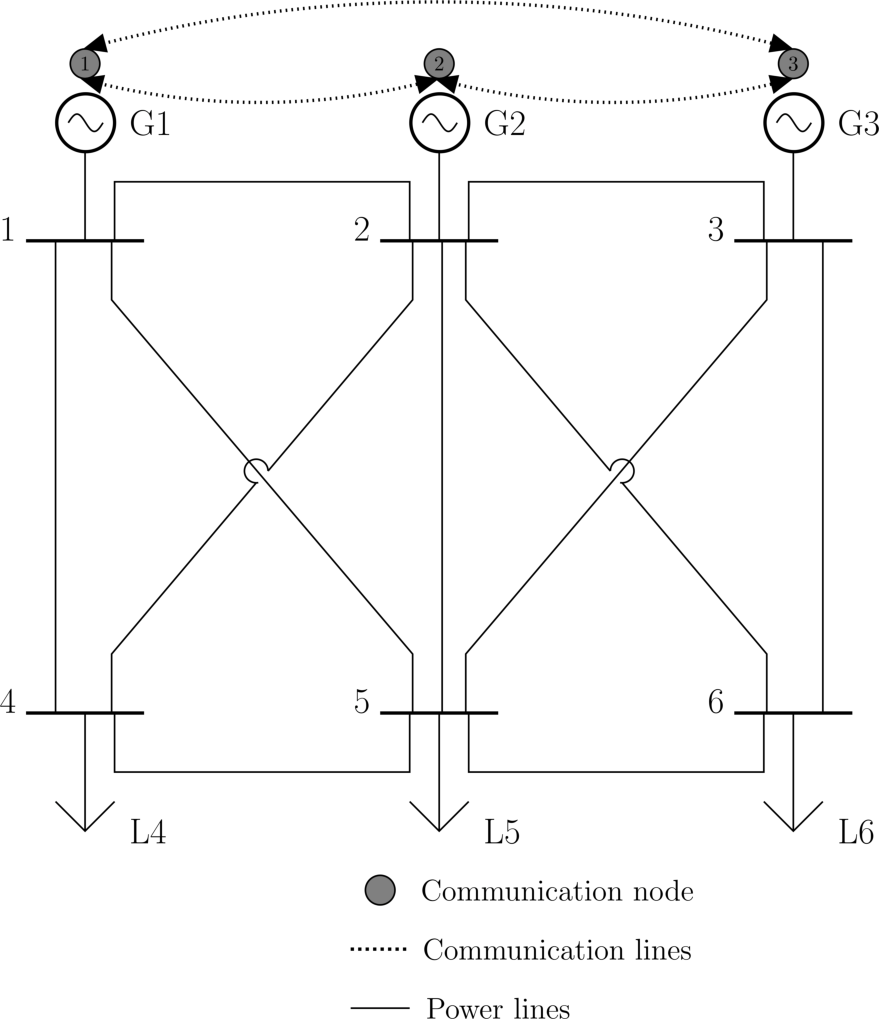
\includegraphics[width=0.4\columnwidth]{images/Six_bus_system.pdf}
	\caption{Single line diagram of six bus system with communication lines}
	\label{fig_six_bus}
\end{figure}
\begin{table}[!ht]
\centering
\begin{tabular}{|c|c|c|c|c|c|} \hline
Generator  &$a_i$  &$b_i$ &$c_i$ &$P_{Gi}^{min}$ &$P_{Gi}^{max}$ \\
bus  &$[\$/MW^2]$ &$[\$/MW]$ &$[\$]$ &$[MW]$ &$[MW]$\\ \hline
1  &213.1  &11.669 &0.00533  &50   &200\\
2  &200    &10.333 &0.00889  &37.5 &150\\
3  &240    &10.833 &0.00741  &45   &180\\ \hline
\end{tabular}
\caption{Generator characteristics of the 6-bus system}
\label{tab_app_1}
\end{table}

\section{Five Bus System}
The single line diagram of five bus microgrid is shown in Fig.~\ref{fig_fivebusMG}. The generator characteristics is given in Table.~\ref{Table.C.2}.
\begin{figure}[!ht]
	\centering
	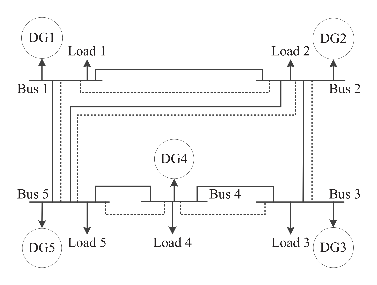
\includegraphics[width=0.5\columnwidth]{images/chapter_6/five_bus_microgrid.eps}
	\caption{Single line diagram of five bus microgrid \cite{wang2018distributed,chen2015distributed}.}
	\label{fig_fivebusMG}
\end{figure}
\begin{table}[!ht]
	\centering
	\begin{tabular}{ccccccc}
			\toprule
			Bus $i$&$c_i$& $b_i$ & $a_i$ & $P_i^{min} (kW)$ &  $P_i^{max} (kW)$ & $P_{di} (kW)$ \\ 
            \midrule
			1	&51	&1.22	&0.094	&10		&80	&35 \\ 
			2	&31	&3.41	&0.078	&8		&60	&20 \\
			3	&78	&2.53	&0.105	&3.8	&40	&25 \\
			4	&42	&4.02	&0.082	&5.4	&45	&30	\\ 	
			5	&62	&3.17	&0.074	&4.2	&18	&10 \\ 
            \bottomrule
	\end{tabular}
	\captionabove{Generator characteristics of five bus microgrid.}
	\label{Table.C.2}
\end{table}

\section{IEEE 39-bus System}
The single line diagram of IEEE 39-bus system is shown in Fig.~\ref{fig:ieee39}. The simulation data is taken from MATPOWER~\cite{zimmerman2010matpower}.

\begin{figure}[!ht]
	\centering
	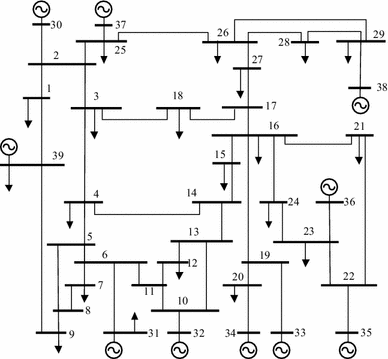
\includegraphics[width=0.7\textwidth]{images/chapter_4/ieee39bus.png}
	\caption{Single line diagram of IEEE 39-bus system \cite{li2014new}}
	\label{fig:ieee39}
\end{figure}

\section{15-node VPP}
The single line diagram of 15-node VPP is shown in Fig.~\ref{fig:15nodeVPP}. The generator characteristics is given in Table.~\ref{Tab_15N_param}.
\begin{table}[!ht]
    \centering
    \begin{tabular}{ccccccc}
        \toprule
        Sl. No. &Bus No. & Type &$b_i$ &$a_i$ &$P_g^\text{min}$ & $P_g^\text{max}$\\
        \midrule
        1 & 4  & DG & $7.2\times10^{-6}$ & 0.031 & 200  & 800 \\
        2 & 6  & DG & $7.5\times10^{-6}$ & 0.029 & 250  & 9000\\
        3 & 8  & DG & $7.3\times10^{-6}$ & 0.030 & 150  & 800 \\
        4 & 10 & ES & $7.6\times10^{-6}$ & 0.027 & -250 & 1000\\
        5 & 13 & ES & $7.5\times10^{-6}$ & 0.028 & -200 & 1000\\
        6 & 5  & IL & $2.4\times10^{-5}$ & 0.012 & 0    & 750\\
        7 & 12 & IL & $2.2\times10^{-5}$ & 0.013 & 0    & 800\\
        \bottomrule
    \end{tabular}
    \captionabove{Cost characteristics and parameters of the DG units}    
    \label{Tab_15N_param}
\end{table}
\begin{figure}[!ht]
	\centering
	\includegraphics[width=0.6\textwidth]{images/chapter_5/15node_vpp.png}
	\caption{Single line diagram of 15-node VPP \cite{mashhour2010bidding,yang2014distributed}}
	\label{fig:15nodeVPP}
\end{figure}


\section{Modified IEEE 33-node System}
The single line diagram of modified IEEE 33-node system is shown in Fig.~\ref{fig:33nodeVPP}. The simulation data is taken from MATPOWER~\cite{zimmerman2010matpower}.

\begin{figure}[!ht]
	\centering
	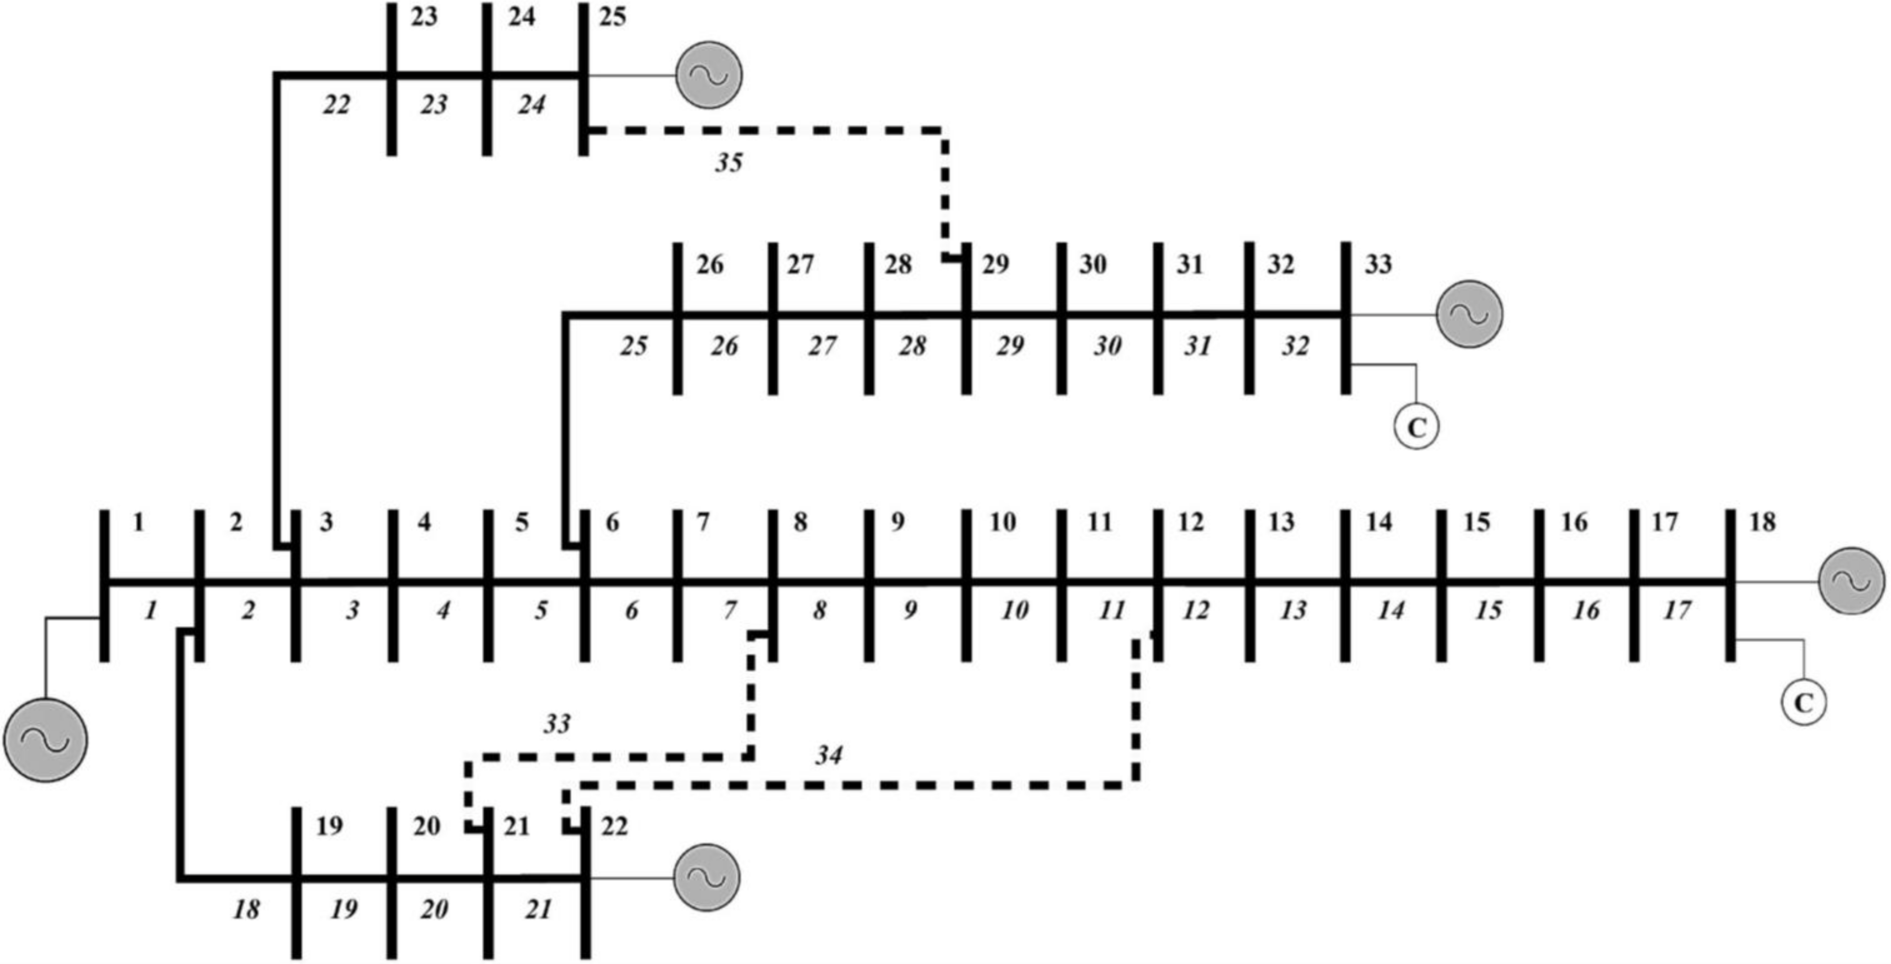
\includegraphics[width=0.95\textwidth]{images/33_node_v1.pdf}
	\caption{Single line diagram of modified IEEE 33-node system~\cite{dolatabadi2020enhanced} }
	\label{fig:33nodeVPP}
\end{figure}

\begin{table}
    \centering
        \begin{tabular}{ccccccc}
            \hline
            bus &b &a &$Pg^\text{min}$ &$Pg^\text{max}$ &$Qg^\text{min}$ &$Qg^\text{max}$ \\ \hline
            1  & 0.5   &$1e^{-6}$     &0     &10   &-10   &10\\
            4  & 0.025 &$0.07e^{-6}$  &0.05  &0.7  &-0.45 &0.45\\
            8  & 0.016 &$0.07e^{-6}$  &0.02  &0.5  &-0.5  &0.5\\
            22 & 0.024 &$0.075e^{-6}$ &0.025 &0.65 &-0.45 &0.45\\
            25 & 0.027 &$0.08e^{-6}$  &0.055 &0.8  &-0.5  &0.5\\
            29 & 0.019 &$0.07e^{-6}$  &0.05  &0.3  &-0.45 &0.45\\ \hline
        \end{tabular}
        \captionabove{Generator characteristics of modified IEEE 33-node system}
\end{table}

